%
% orthogonal.tex
%
% (c) 2021 Prof Dr Andreas Müller, OST Ostschweizer Fachhochschule
%
\section{Orthogonale Funktionenfamilien
\label{buch:orthogonalitaet:section:orthogonale-funktionen}}
\rhead{Orthogonale Funktionenfamilien}
Die Fourier-Theorie basiert auf der Idee, Funktionen durch 
Funktionenreihen mit Summanden zu bilden, die im Sinne eines
Skalarproduktes orthogonal sind, welches mit Hilfe eines Integrals
definiert sind.
Solche Funktionenfamilien treten jedoch auch als Lösungen von
Differentialgleichungen auf.
Besonders interessant wird die Situation, wenn die Funktionen 
Polynome sind.
In diesem Abschnitt soll zunächst das Skalarprodukt definiert 
und an Hand von Beispielen gezeigt werden, wie verschiedenartige
interessante Familien von orthogonalen Polynomen gewonnen werden
können.

%
% Skalarprodukt
%
\subsection{Skalarprodukt}
Der reelle Vektorraum $\mathbb{R}^n$ trägt das Skalarprodukt
\[
\langle\;\,,\;\rangle
\colon
\mathbb{R}^n \times \mathbb{R}^n \to \mathbb{R}
:
(x,y)\mapsto \langle x, y\rangle = \sum_{k=1}^n x_iy_k,
\]
welches viele interessante Anwendungen ermöglicht.
Eine orthonormierte Basis macht es zum Beispiel besonders leicht,
eine Zerlegung eines Vektors in dieser Basis zu finden.
In diesem Abschnitt soll zunächst an die Eigenschaften erinnert
werden, die zu einem nützlichen 

\subsubsection{Eigenschaften eines Skalarproduktes}
Das Skalarprodukt erlaubt auch, die Länge eines Vektors $v$
als $|v| = \sqrt{\langle v,v\rangle}$ zu definieren.
Dies funktioniert natürlich nur, wenn die Wurzel auch immer
definiert ist, d.~h.~das Skalarprodukt eines Vektors mit sich
selbst darf nicht negativ sein.
Dazu dient die folgende Definition.

\begin{definition}
Sei $V$ ein reeller Vektorraum.
Eine bilineare Abbildung
\[
\langle\;\,,\;\rangle
\colon
V\times V
\to
\mathbb{R}
:
(u,v) \mapsto \langle u,v\rangle.
\]
heisst {\em positiv definit}, wenn für alle Vektoren $v \in V$ mit
$v\ne 0 \Rightarrow \langle v,v\rangle > 0$ 
Die {\em Norm} eines Vektors $v$ ist
$|v|=\sqrt{\langle v,v\rangle}$.
\end{definition}

Damit man mit dem Skalarprodukt sinnvoll rechnen kann, ist ausserdem
erforderlich, dass es eine einfache Beziehung zwischen 
$\langle x,y\rangle$ und $\langle y,x\rangle$ gibt.

\begin{definition}
Ein {\em Skalarprodukt} auf einem reellen Vektorraum $V$ ist eine
positiv definite, symmetrische bilineare Abbildung
\[
\langle\;\,,\;\rangle
\colon
V\times V
\to
\mathbb{R}
:
(u,v) \mapsto \langle u,v\rangle.
\]
\end{definition}

Das Skalarprodukt $\langle u,v\rangle=u^tv$ auf dem Vektorraum 
$\mathbb{R}^n$ erfüllt die Definition ganz offensichtlich,
sie führt auf die Komponentendarstellung
\[
\langle u,v\rangle = u^tv = \sum_{k=1}^n u_iv_i.
\]
Weitere Skalarprodukte ergeben ergeben sich mit jeder symmetrischen,
positiv definiten Matrix $G$ und der Definition
$\langle u,v\rangle_G=u^tGv$.
Ein einfacher Spezialfall tritt auf, wenn $G$ eine Diagonalmatrix
$\operatorname{diag}(w_1,\dots,w_n)$
mit positiven Einträgen $w_i>0$ auf der Diagonalen ist.
In diesem Fall schreiben wir
\[
\langle u,v\rangle_w
=
u^t\operatorname{diag}(w_1,\dots,w_n)v
=
\sum_{k=1}^n u_iv_i\,w_i
\]
und nennen $\langle \;\,,\;\rangle_w$ das {\em gewichtete Skalarprodukt}
mit {\em Gewichten $w_i$}.

\subsubsection{Skalarprodukte auf Funktionenräumen}
Das Integral ermöglicht jetzt, ein Skalarprodukt auf dem reellen
Vektorraum der stetigen Funktionen auf einem Intervall zu definieren.

\begin{definition}
\label{buch:orthogonal:def:skalarprodukt}
Sei $V$ der reelle Vektorraum $C([a,b])$ der reellwertigen, stetigen
Funktion auf dem Intervall $[a,b]$.
Dann ist 
\[
\langle\;\,,\;\rangle
\colon
C([a,b]) \times C([a,b]) \to \mathbb{R}
:
(f,g) \mapsto \langle f,g\rangle = \int_a^b f(x)g(x)\,dx.
\]
ein Skalarprodukt.
\end{definition}

Die Definition ist offensichtlich symmetrisch in $f$ und $g$ und
aus den Eigenschaften des Integrals ist klar, dass das Produkt
bilinear ist:
\begin{align*}
\langle \lambda_1 f_1+\lambda_2f_2,g\rangle
&=
\int_a^b (\lambda_1f_(x) +\lambda_2f_2(x))g(x)\,dx
=
\lambda_1\int_a^b f_1(x) g(x)\,dx
+
\lambda_2\int_a^b f_2(x) g(x)\,dx
\\
&=
\lambda_1\langle f_1,g\rangle
+
\lambda_2\langle f_2,g\rangle.
\end{align*}
Ausserdem ist es positiv definit, denn wenn $f(x_0) \ne 0$ ist,
dann gibt es wegen der Stetigkeit von $f$ eine Umgebung
$U=[x_0-\varepsilon,x_0+\varepsilon]$, derart, dass $|f(x)| > \frac12|f(x_0)|$
ist für alle $x\in U$.
Somit ist das Integral
\[
\langle f,f\rangle
=
\int_a^b |f(x)|^2\,dx
\ge
\int_{x_0-\varepsilon}^{x_0+\varepsilon} |f(x)|^2\,dx
\ge
\int_{x_0-\varepsilon}^{x_0+\varepsilon} \frac14|f(x_0)|^2\,dx
=
\frac{1}{4}|f(x_0)|^2\cdot 2\varepsilon
=
\frac{|f(x_0)|^2\varepsilon}{2}
>0,
\]
was beweist, dass $\langle\;,\;\rangle$ positiv definit und damit
ein Skalarprodukt ist.

Die Definition kann noch etwas verallgemeinert werden, indem 
die Funktionswerte nicht überall auf dem Definitionsbereich 
gleich gewichtet werden. 

\begin{definition}
\label{buch:orthogonal:def:skalarproduktw}
Sei $w\colon [a,b]\to \mathbb{R}^+$ eine positive, stetige Funktion,
dann ist
\[
\langle\;\,,\;\rangle_w
\colon
C([a,b]) \times C([a,b]) \to \mathbb{R}
:
(f,g) \mapsto \langle f,g\rangle_w = \int_a^b f(x)g(x)\,w(x)\,dx.
\]
das {\em gewichtete Skalarprodukt} mit {\em Gewichtsfunktion $w(x)$}.
\end{definition}

\subsection{Gram-Schmidt-Orthonormalisierung}
In einem reellen Vektorraum $V$ mit Skalarprodukt $\langle\;\,,\;\rangle$
kann aus einer beleibigen Basis $b_1,\dots,b_n$ mit Hilfe des 
Gram-Schmidtschen Orthogonalisierungsverfahrens immer eine
orthonormierte Basis $\tilde{b}_1,\dots,\tilde{b}_n$ Basis
gewonnen werden.
Es stellt sicher, dass für alle $k\le n$ gilt
\[
\langle b_1,\dots,b_k\rangle
=
\langle \tilde{b}_1,\dots,\tilde{b}_k\rangle.
\]
Zur Vereinfachung der Formeln schreiben wir $v^0=v/|v|$ für einen zu
$v$ parallelen Einheitsvektor.
Die Vektoren $\tilde{b}_i$ können mit Hilfe der Formeln
\begin{align*}
\tilde{b}_1
&=
(b_1)^0
\\
\tilde{b}_2
&=
\bigl(
b_2
-
\langle \tilde{b}_1,b_2\rangle \tilde{b}_1
\bigr)^0
\\
\tilde{b}_3
&=
\bigl(
b_3
-
\langle \tilde{b}_1,b_3\rangle \tilde{b}_1
-
\langle \tilde{b}_2,b_3\rangle \tilde{b}_2
\bigr)^0
\\
&\;\vdots
\\
\tilde{b}_n
&=
\bigl(
b_n
-
\langle \tilde{b}_1,b_n\rangle \tilde{b}_1
-
\langle \tilde{b}_2,b_n\rangle \tilde{b}_2
-\dots
-
\langle \tilde{b}_{n-1},b_n\rangle \tilde{b}_{n-1}
\bigr)^0
\end{align*}
iterativ berechnet werden.
Dieses Verfahren lässt sich auch auf Funktionenräume anwenden.

Die Normierung ist nicht unbedingt nötig und manchmal unangenehm,
da die Norm unschöne Quadratwurzeln einführt.
Falls es genügt, eine orthogonale Basis zu finden, kann darauf
verzichtet werden, bei der Orthogonalisierung muss aber berücksichtigt
werden, dass die Vektoren $\tilde{b}_i$ jetzt nicht mehr Einheitslänge
haben.
Die Formeln
\begin{align*}
\tilde{b}_0
&=
b_0
\\
\tilde{b}_1
&=
b_1
-
\frac{\langle b_1,\tilde{b}_0\rangle}{\langle \tilde{b}_0,\tilde{b}_0\rangle}\tilde{b}_0
\\
\tilde{b}_2
&=
b_2
-
\frac{\langle b_2,\tilde{b}_0\rangle}{\langle \tilde{b}_0,\tilde{b}_0\rangle}\tilde{b}_0
-
\frac{\langle b_2,\tilde{b}_1\rangle}{\langle \tilde{b}_1,\tilde{b}_1\rangle}\tilde{b}_1
\\
&\;\vdots
\\
\tilde{b}_n
&=
b_n
-
\frac{\langle b_n,\tilde{b}_0\rangle}{\langle \tilde{b}_0,\tilde{b}_0\rangle}\tilde{b}_0
-
\frac{\langle b_n,\tilde{b}_1\rangle}{\langle \tilde{b}_1,\tilde{b}_1\rangle}\tilde{b}_1
-
\dots
-
\frac{\langle b_n,\tilde{b}_{n-1}\rangle}{\langle \tilde{b}_{n-1},\tilde{b}_{n-1}\rangle}\tilde{b}_{n-1}.
\end{align*}
berücksichtigen dies.

%
% Legendre-Polynome
%
\subsection{Legendre-Polynome
\label{buch:orthogonal:subsection:legendre-polynome}}
Der Gram-Schmidtsche Orthogonalisierungsprozess kann für jedes beliebige
Skalarprodukt aus der Folge $1$, $x$, $x^2,\dots$ der Monome ein
Folge von orthogonalisierten Polynomen machen.
In diesem Abschnitt rechnen wir den Fall konstanter Gewichtsfunktione
$w(x)=1$ durch, er führt auf die sogenannten {\em Legendre-Polynome}.

Da wir auf die Normierung verzichten, brauchen wir ein anderes
Kriterium, welches die Polynome eindeutig festlegen kann.
Wir bezeichnen das Polynom vom Grad $n$, das bei diesem Prozess
entsteht, mit $P_n(x)$ und legen willkürlich aber traditionskonform
fest, dass $P_n(1)=1$ sein soll.

%
% Symmetrie-Eigenschaften
%
\subsubsection{Symmetrieeigenschaften}
Das Skalarprodukt berechnet ein Integral eines Produktes von zwei
Polynomen über das symmetrische Interval $[-1,1]$.
Ist die eine gerade und die andere ungerade, dann ist das
Produkt eine ungerade Funktion und das Skalarprodukt verschwindet.
Sind beide Funktionen gerade oder ungerade, dann ist das Produkt
gerade und das Skalarprodukt ist im Allgmeinen von $0$ verschieden.
Dies zeigt, dass es tatsächlich etwas zu Orthogonalisieren gibt.

Die ersten beiden Funktionen sind das konstante Polynom $1$ und
das Polynome $x$.
Nach obiger Beobachtung ist das Skalarprodukt $\langle 1,x\rangle=0$,
also ist $P_1(x)=x$.
Die Graphen der entstehenden Polynome sind in
Abbildung~\ref{buch:integral:orthogonal:legendregraphen}
dargestellt.
\begin{figure}
\centering
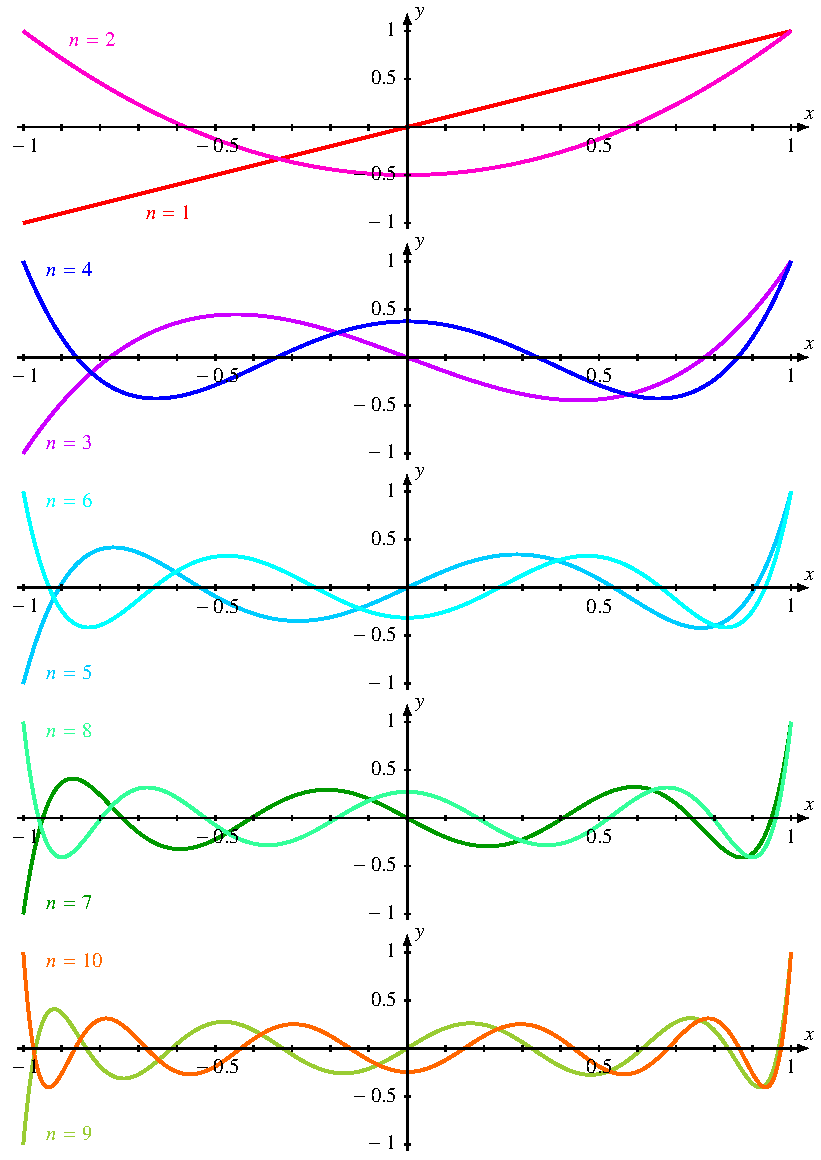
\includegraphics{chapters/070-orthogonalitaet/images/legendre.pdf}
\caption{Graphen der Legendre-Polynome $P_n(x)$ für $n=1,\dots,10$.
\label{buch:integral:orthogonal:legendregraphen}}
\end{figure}

\begin{lemma}
\label{buch:orthogonal:lemma:symmetrie}
Die Polynome $P_{2n}(x)$ sind gerade, die Polynome $P_{2n+1}(x)$ sind
ungerade Funktionen von $x$.
\end{lemma}

\begin{proof}[Beweis]
Wir verwenden vollständige Induktion nach $n$.
Wir wissen bereits, dass $P_0(x)=1$ und $P_1(x)=x$ die verlangten
Symmetrieeigenschaften haben.
Im Sinne der Induktionsannahme nehmen wir daher an, dass die
Symmetrieeigenschaften für $P_k(x)$, $k<n$, bereits bewiesen sind.
$P_n(x)$ entsteht jetzt durch Orthogonalisierung nach der Formel
\[
P_n(x)
=
x^n
-
\langle P_{n-1},x^n\rangle P_{n-1}(x)
-
\langle P_{n-2},x^n\rangle P_{n-2}(x)
-\dots-
\langle P_1,x^n\rangle P_1(x)
-
\langle P_0,x^n\rangle P_0(x).
\]
Die Skalarprodukte
$\langle P_{n-1},x^n\rangle$,
$\langle P_{n-3},x^n\rangle$, $\dots$ verschwinden alle, so dass
$P_n(x)$ eine Linearkombination der Funktionen $x^n$, $P_{n-2}(x)$,
$P_{n-4}(x)$ ist, die die gleiche Parität wie $x^n$ haben.
Also hat auch $P_n(x)$ die gleiche Parität, was das Lemma beweist.
\end{proof}

%
% Orthogonalisierung nach Gram-Schmidt
%
\subsubsection{Orthogonalisierung mit Gram-Schmidt}
Die Ortogonalisierung von $x^2$ liefert daher
\[
p(x) = x^2
-
\frac{\langle x^2,P_0\rangle}{\langle P_0,P_0\rangle} P_0(x)
=
x^2 - \frac{\int_{-1}^1x^2\,dx}{\int_{-1}^11\,dx}
=
x^2 - \frac{\frac{2}{3}}{2}=x^2-\frac13
\]
Dieses Polynom erfüllt die Standardisierungsbedingung noch 
nicht den $p(1)=\frac23$.
Daraus leiten wir ab, dass
\[
P_2(x) = \frac12(3x^2-1)
\]
ist.

Für $P_3(x)$ brauchen wir nur die Skalaprodukte
\[
\left.
\begin{aligned}
\langle x^3,P_1\rangle
&=
\int_{-1}^1  x^3\cdot x\,dx
=
\biggl[\frac15x^5\biggr]_{-1}^1
=
\frac25
\qquad
\\
\langle P_1,P_1\rangle
&=
\int_{-1}^1 x^2\,dx
=
\frac23
\end{aligned}
\right\}
\qquad
\Rightarrow
\qquad
p(x) = x^3 - \frac{\;\frac25\;}{\frac23}x=x^3-\frac{3}{5}x
\]
Die richtige Standardisierung ergibt sich,
indem man durch $p(1)=\frac25$ dividiert, also
\[
P_2(x) = \frac12(5x^3-3x).
\]

Die Berechnung weiterer Polynome verlangt, dass Skalarprodukte
$\langle x^n,P_k\rangle$ berechnet werden müssen, was wegen
der zunehmend komplizierten Form von $P_k$ etwas mühsam ist.
Wir berechnen den Fall $P_4$.
Dazu muss das Polynom $x^4$ um eine Linearkombination von
$P_2$ und $P_0(x)=1$ korrigiert werden.
Die Skalarprodukte sind
\begin{align*}
\langle x^4, P_0\rangle
&=
\int_{-1}^1 x^4\,dx = \frac25
\\
\langle P_0,P_0\rangle
&=
\int_{-1}^1 \,dx = 2
\\
\langle x^4,P_2\rangle
&=
\int_{-1}^1 \frac32x^6-\frac12 x^4\,dx
=
\biggl[\frac{3}{14}x^7-\frac{1}{10}x^5\biggr]_{-1}^1
=
\frac6{14}-\frac15
=
\frac8{35}
\\
\langle P_2,P_2\rangle
&=
\int_{-1}^1 \frac14(3x^2-1)^2\,dx
=
\int_{-1}^1 \frac14(9x^4-6x^2+1)\,dx
=
\frac14\biggl(\frac{18}{5}-4+2\biggr)
=\frac25.
\end{align*}
Daraus folgt für $p(x)$
\begin{align*}
p(x)
&=
x^4
-
\frac{\langle x^4,P_2\rangle}{\langle P_2,P_2\rangle}P_2(x)
-
\frac{\langle x^4,P_0\rangle}{\langle P_0,P_0\rangle}P_0(x)
\\
&=
x^4
-\frac47 P_2(x) - \frac15 P_0(x)
\\
&=
x^4 - \frac{6}{7}x^2 + \frac{3}{35}
\end{align*}
mit $p(1)=\frac{8}{35}$, so dass man
\[
P_4(x) =
\frac18(35x^4-30x^2+3)
\]
setzen muss.

\begin{figure}
\centering
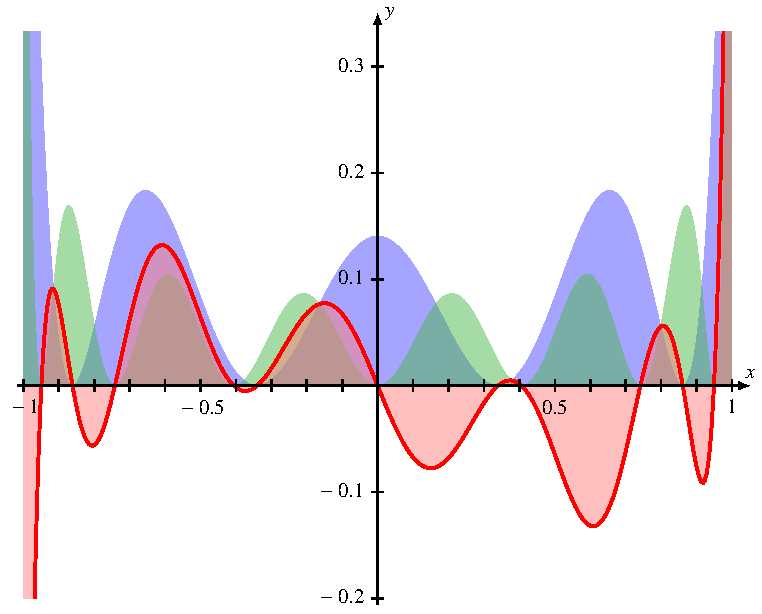
\includegraphics{chapters/070-orthogonalitaet/images/orthogonal.pdf}
\caption{Orthogonalität der Legendre-Polynome $P_4(x)$ ({\color{blue}blau})
und $P_7(x)$ ({\color{darkgreen}grün}).
Die blaue Fläche ist die Fläche unter dem Graphen 
von $P_4(x)^2$, $P_4(x)$ muss durch die Wurzel aus diesem Flächeninhalt
geteilt werden, um ein Polynome mit Norm $1$ zu erhalten.
Für die grüne Fläche ist es $P_7(x)$.
Die rote Kurve ist der Graph der Funktion $P_4(x)\cdot P_7(x)$,
die rote Fläche ist deren Integral, sie ist $0$, d.~h.~die beiden
Funktionen sind orthogonal.
\label{buch:integral:orthogonal:legendreortho}}
\end{figure}

\begin{table}
\centering
\renewcommand{\arraystretch}{1.2}
\begin{tabular}{|>{$}c<{$}|>{$}l<{$}|}
\hline
n&P_n(x)\\
\hline
 0&1
\\
 1&x
\\
 2&\frac12(3x^2-1)
\\
 3&\frac12(5x^3-3x)
\\
 4&\frac18(35x^4-30x^2+3)
\\
 5&\frac18(63x^5-70x^3+15x)
\\
 6&\frac1{16}(231x^6-315x^4+105x^2-5)
\\
 7&\frac1{16}(429x^7-693x^5+315x^3-35x)
\\
 8&\frac1{128}(6435x^8-12012x^6+6930x^4-1260x^2+35)
\\
 9&\frac1{128}(12155x^9-25740x^7+18018x^5-4620x^3+315x)
\\
10&\frac1{256}(46189x^{10}-109395x^8+90090x^6-30030x^4+3465x^2-63)
\\[2pt]
\hline
\end{tabular}
\caption{Die Legendre-Polynome $P_n(x)$ für $n=0,1,\dots,10$ sind
orthogonale Polynome vom Grad $n$, die den Wert $P_n(1)=1$ haben.
\label{buch:integral:table:legendre-polynome}}
\end{table}

Die so konstruierten Polynome heissen die {\em Legendre-Polynome}.
Durch weitere Durchführung des Verfahrens liefert die Polynome in
Tabelle~\ref{buch:integral:table:legendre-polynome}.
Die Graphen sind in Abbildung~\ref{buch:integral:orthogonal:legendregraphen}
dargestellt.
Abbildung~\ref{buch:integral:orthogonal:legendreortho} illustriert, 
dass die beiden Polynome $P_4(x)$ und $P_7(x)$ orthogonal sind.
Das Produkt $P_4(x)\cdot P_7(x)$ hat Integral $=0$.

%
% Verschiedene Gewichtsfunktionen
%
\subsection{Gewichtsfunktionen
\label{buch:orthogonal:subsection:gewichtsfunktionen}}
Das Standardskalarprodukt auf dem Raum der Funktionen auf dem
Interval $[-1,1]$ ist das Skalarprodukt mit der Gewichtsfunktion
$w(x)=1$, es führt auf die Legendre-Polynome.
Die Wahl einer anderen Gewichtsfunktion ändert natürlich
das Resultat der Orthogonalisierung.
Nullstellen und Pole der Gewichtsfunktion ändern die Menge der
Funktionen, für die das Skalarprodukt definiert.
Diesem Zusammenhang soll im ersten Unterabschnitt nachgegangen werden.
Danach sollen verschiedene für die Praxis relevante Gewichtsfunktionen
vorgestellt werden.

\begin{figure}
\centering
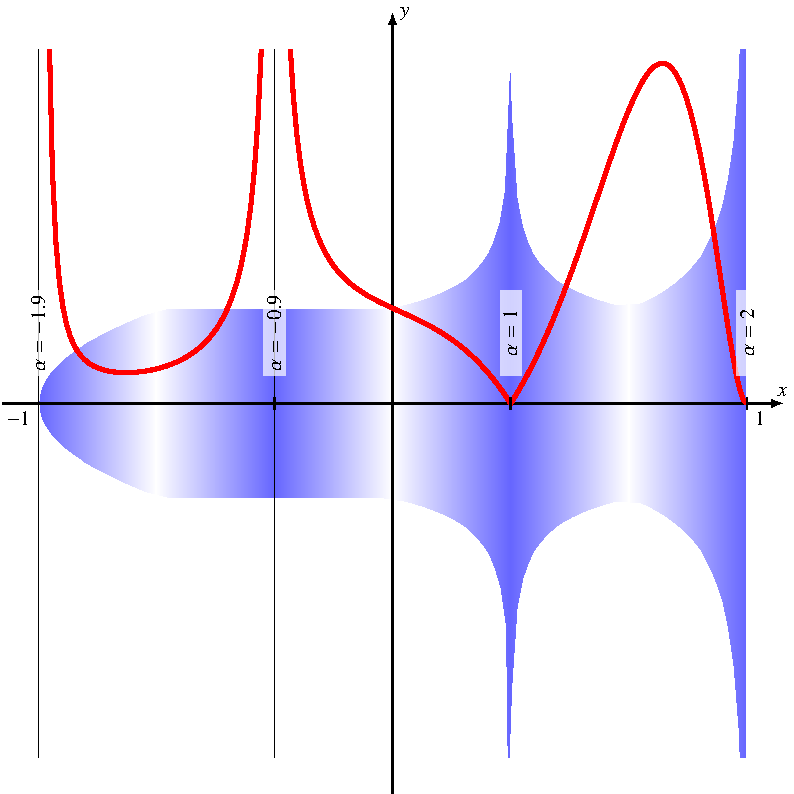
\includegraphics{chapters/070-orthogonalitaet/images/weight.pdf}
\caption{Nullstellen und Pole der Gewichtsfunktion (rot) legen Ort
und Grad von Polen und Nullstellen der Funktionen fest, die beschränkte
$\|\,\cdot\,\|_w$-Norm haben.
An den Stellen $\pm 1$ und $\pm\frac12$ hat die Gewichtsfunktion
Pole bzw.~Nullstellen mit Grad $\alpha$.
Der blaue Bereich deutet an, wie schnell die Funktion $f$ in diesem
Bereich anwachsen kann, bzw.~wie schnell nahe der Polstelle gegen $0$
gehen muss.
\label{buch:orthogonalitaet:fig:gewicht}}
\end{figure}
%
% Pole und Nullstellen der Gewichtsfunktion
%
\subsubsection{Pole und Nullstellen
\label{buch:orthogonal:pole-und-nullstellen}}
Das Skalarprodukt $\langle\,\;,\;\rangle_w$ ist nur sinnvoll
für Funktionen $f(x)$, für die die Norm $\|f\|_w$ definiert ist.
An einer Nullstelle $x_0$ der Gewichtsfunktion $w$ darf die Funktion $f$ 
einen Pol haben. 
Solange $f(x)$ für $x\to x_0$ nicht zu schnell divergiert, kann
das Produkt $|f(x)|^2 w(x)$ immer noch integrierbar sein.

Um dies etwas genauer zu quantifizieren, nehmen wir an, dass
$w(x)$ an der Stelle $x_0$ eine Nullstelle vom Grad $\alpha$ hat.
Dies bedeutet, dass $w(x) \approx C|x-x_0|^\alpha$ ist für eine geeignete
Konstante $C$ und für $|x-x_0|<\varepsilon$.
Ein Pol von $f$ vom Grad $a$ an der Stelle $x_0$ führt entsprechend auf
eine Abschätzung $|f(x)| \approx D|f(x)|^{-a}$ für $|x-x_0|<\varepsilon$.
Dann ist
\[
|f(x)|^2 w(x) \approx CD |x-x_0|^{\alpha-2a}.
\]
Für das Integral in der Nähe von $x_0$ ist
\begin{align*}
\int_{x_0-\varepsilon}^{x_0+\varepsilon}
|f(x)|^2 w(x)\,dx
&\approx 
CD
\int_{x_0-\varepsilon}^{x_0+\varepsilon}
|x-x_0|^{\alpha-2a}\,dx
\\
&=
2CD
\int_0^\varepsilon
t^{\alpha-2a}
\,dt
=
2CD
\begin{cases}
\displaystyle
\;
\biggl[\frac{t^{\alpha-2a+1}}{\alpha-2a+1}\biggr]_0^\varepsilon
&\qquad
\alpha-2a\ne-1
\\[7pt]
\displaystyle
\;
\biggl[ \log t \biggr]_0^\varepsilon
&\qquad
\text{sonst.}
\end{cases}
\end{align*}
Der Zähler $t^{\alpha-2a+1}$ divergiert für $t\to 0$ genau dann,
wenn $\alpha-2a+1<0$ oder $\alpha<2a-1$.
Auch im zweiten Fall, für $\alpha-2a+1=0$, divergiert das Integral.
Damit die Norm $\|f\|_w$ definiert ist, muss also $a<\frac12(\alpha+1)$
sein.

Ganz ähnlich führt eine Polstelle von $w$ vom Grad $\alpha$
an der Stelle $x_0$ dazu, dass $f$ dort eine Nullstelle vom Grad
$a$ haben muss.
Das Normintegral konvergiert nur, wenn $2a-\alpha > -1$ ist
oder $a > \frac12(\alpha+1)$.
 
Pole der Gewichtsfunktion schränken also ein, welche Funktionen
überhaupt der Untersuchung mit Hilfe des Skalarproduktes
$\langle\,\;,\;\rangle_w$ zugänglich sind
(Abbildung~\ref{buch:orthogonalitaet:fig:gewicht}).
Ist die Ordnung $\alpha$ des Poles grösser als $1$, dann müssen die Funktionen
eine Nullstelle mindestens vom Grad $\frac12(a+1)$ haben.
Nullstellen der Gewichtsfunktion erweitern die Klasse der Funktionen.
Ist die Ordnung der Nullstelle $\alpha$, dann dürfen die Funktionen einen
Pol der Ordnung kleiner als $\frac12(\alpha+1)$ haben.

\begin{lemma}
\label{buch:orthogonal:lemma:gewichtsfunktion}
Sei $w(x)\ge 0$ auf dem Intervall $(a,b)$.
Der Vektorraum $H_w$ von auf $(a,b)$ definierten Funktionen sei
\[
H_w
=
\biggl\{
f\colon(a,b) \to \mathbb{R}
\;\bigg|\;
\int_a^b |f(x)|^2 w(x)\,dx
\biggr\}.
\]
Die Funktionen $f\in H_w$ haben folgende Eigenschaften
\begin{enumerate}
\item
Ist $\xi\in[a,b]$ eine Nullstelle vom Grad $\alpha$ der Funktion $w(x)$,
dann 
\item
Ist $\xi\in[a,b]$ eine Polstelle vom Grad $a$ der Funktion $w(x)$,
dann hat $f$ eine Nullstelle mindestens from Grad 
\end{enumerate}
\end{lemma}


%
% Die Jacobische Gewichtsfunktion
%
\subsubsection{Jacobische Gewichtsfunktion}
Die Gewichtsfunktion für die Legendre-Polynome war $w(x)=1$, alle
Punkte im Intervall $(-1,1)$ hatten das gleiche Gewicht.
Diese soll jetzt ersetzt werden durch eine Gewichtsfunktion, die
den Punkten an den Intervallenden mehr oder weniger Gewicht gibt,
wobei auch zugelassen sein soll, dass die Gewichtung nicht symmetrisch
ist.

\begin{definition}
\label{buch:orthogonal:def:jacobi-gewichtsfunktion}
Die {\em Jacobi-Gewichtsfunktion} ist die Funktion
\index{Jacobi-Gewichtsfunktion}%
\[
w^{(\alpha,\beta)}
\colon (-1,1)\to\mathbb{R}
:
x\mapsto w^{(\alpha,\beta)}(x) = (1-x)^\alpha(1+x)^\beta
\]
mit $\alpha,\beta\in\mathbb{R}$.
Das Skalarprodukt zugehörige Skalarprodukt wird auch als
\[
\langle\,\;,\;\rangle_{w^{(\alpha,\beta)}}
=
\langle\,\;,\;\rangle_{(\alpha,\beta)}
\]
bezeichnet und die zugehörige Norm mit
\[
\|f\|_{(\alpha,\beta)}
=
\langle f,f\rangle_{(\alpha,\beta)}
=
\int_{-1}^1 |f(x)|^2 w^{(\alpha,\beta)}(x)\,dx.
\]
\end{definition}

\begin{definition}
\label{buch:orthogonal:def:jacobi-polynome}
Die {\em Jacobi-Polynome} $P^{(\alpha,\beta)}_n(x)$ sind 
\index{Jacobi-Polynome}%
Polynome vom Grad $n$, die bezüglich des Skalarproduktes
$\langle\,\;,\;\rangle_{w^{(\alpha,\beta)}}$ orthogonal sind
und mit
\[
P_n^{(\alpha,\beta)}(1) = \binom{n+\alpha}n
\]
normiert sind.
\end{definition}

In Abbildung~\ref{buch:orthogonal:fig:jacobi-parameter}
ist die Abhängigkeit der Jacobi-Polynome von den Parametern $\alpha$
und $\beta$ illustriert.
Für $\alpha=\beta=0$ entsteht die Gewichtsfunktion
$w^{(0,0)}(x)=1$, die Legendre-Polynome sind also der Spezialfall
$\alpha=\beta=0$ der Jacobi-Polynome.

Der Exponent $\alpha$ in der Gewichtsfunktion $w^{(\alpha,\beta)}(x)$
steuert das Gewicht, welches Punkte am rechten Rand des Intervalls
erhalten.
Für positive Werte von $\alpha$ hat $w^{(\alpha,\beta)}(x)$ eine
Nullstelle vom Grad $\alpha$ an der Stelle $x=1$, nach
Lemma~\ref{buch:orthogonal:lemma:gewichtsfunktion}
dürfen die Funktionen einen Pole der Ordnung $<\frac12(\alpha-1)$ haben.
Je grösser $\alpha$ ist, desto weniger Gewicht haben die Punkte
am rechten Rand des Intervalls und desto schneller darf eine Funktion
für $x\to 1$ divergieren.

Für negative Werte von $\alpha$ hat $w^{(\alpha,\beta)}(x)$ einen
Pol vom Grad $-\alpha$ an der Stelle $x=1$.
Funktionen müssen daher also ein Nullstelle mindestens vom Grad
$\frac12(1-\alpha)$ haben.

\begin{figure}
\centering
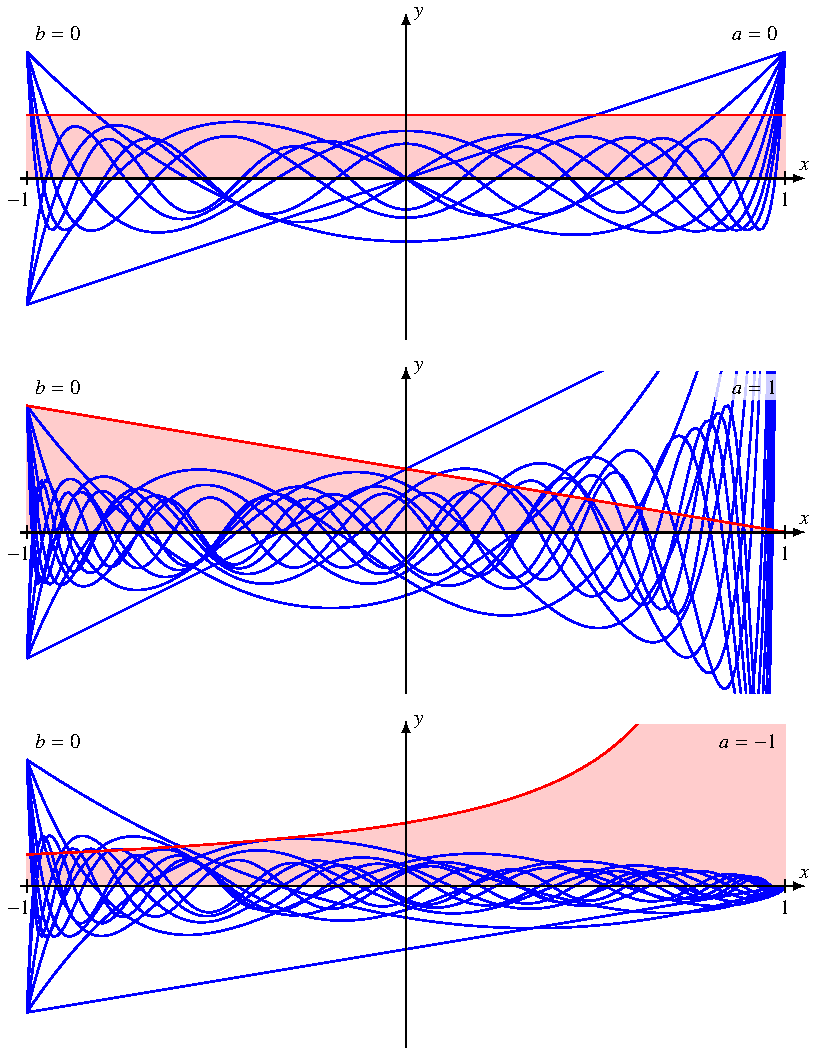
\includegraphics[width=\textwidth]{chapters/070-orthogonalitaet/images/jacobi.pdf}
\caption{Jacobi-Polynome vom Grad $1$ bis $14$ für verschiedene Werte
der Parameter $\alpha$ und $\beta$.
Je grösser $\alpha$, desto weniger Gewicht bekommen die Funktionswerte am
rechten Rand und desto grösser werden die Funktionswerte.
Für negative $\alpha$ müssen die Polynome dagegen eine Nullstelle am
rechten Rand haben.
\label{buch:orthogonal:fig:jacobi-parameter}}
\end{figure}

\subsubsection{Jacobi-Gewichtsfunktion und Beta-Verteilung
\label{buch:orthogonal:subsection:beta-verteilung}}
Die Jacobi-Gewichtsfunktion entsteht aus der Wahrscheinlichkeitsdichte
der Beta-Verteilung, die in
Abschnitt~\ref{buch:rekursion:subsection:beta-verteilung}
eingeführt wurde mit Hilfe der Variablen-Transformation $x = 2t-1$
oder $t=(x+1)/2$.
Das Integral mit der Jacobi-Gewichtsfunktion $w^{(\alpha,\beta)}(x)$
kann damit umgeformt werden in
\begin{align*}
\int_{-1}^1
f(x)\,w^{(\alpha,\beta)}(x)\,dx
&=
\int_0^1
f(2t-1) w^{(\alpha,\beta)}(2t-1)\,2\,dt
\\
&=
\int_0^1
f(2t-1)
(1-(2t-1))^\alpha (1+(2t-1))^\beta
\,2\,dt
\\
&=
2^{\alpha+\beta+1}
\int_0^1
f(2t-1)
\,
t^\beta
(1-t)^\alpha
\,dt
\\
&=
2^{\alpha+\beta+1}
B(\alpha+1,\beta+1)
\int_0^1
f(2t-1)
\,
\frac{
t^\beta
(1-t)^\alpha
}{B(\alpha+1,\beta+1)}
\,dt.
\end{align*}
Auf der letzten Zeile steht ein Integral mit der Wahrscheinlichkeitsdichte
der Beta-Verteilung.
Orthogonale Funktionen bezüglich der Jacobischen Gewichtsfunktion
$w^{(\alpha,\beta)}$ werden mit der genannten Substitution also
zu orthogonalen Funktionen bezüglich der Beta-Verteilung mit
Parametern $\beta+1$ und $\alpha+1$.


%
% Tschebyscheff-Gewichtsfunktion
%
\subsubsection{Tschebyscheff-Gewichtsfunktion}
Es wird später gezeigt werden, dass die Tschebyscheff-Polynome
von Abschnitt~\ref{buch:polynome:section:tschebyscheff} eine
Familie orthogonaler Polynome sein.
Das zugehörige Skalarprodukt hat die Gewichtsfunktion
\[
w_{\text{Tschebyscheff}}(x)
=
\frac{1}{\sqrt{1-x^2}}
=
\frac{1}{\sqrt{(1-x)(1+x)}}
=
(1-x)^{-\frac{1}{2}}
(1+x)^{-\frac{1}{2}}
=
w^{(-\frac12,-\frac12)}(x).
\]
Die {\em Tschebyscheff-Gewichtsfunktion} ist also ein Spezialfall der
Jacobi-Gewichtsfunktion.
\index{Tschebyscheff-Gewichtsfunktion}%

%
% Hermite-Gewichtsfunktion
%
\subsubsection{Hermite-Gewichtsfunktion}
Die Gewichtsfunktion
\[
w_{\text{Hermite}}(x)
=
w(x)
=
e^{-\frac{x^2}{2}}
\]
heisst die {\em Hermite-Gewichtsfunktion}.
\index{Hermite-Gewichtsfunktion}%
Sie hat keine Nullstellen und geht für $x\to\pm\infty$ so schnell
gegen $0$, dass für alle Polynome 
\[
\int_{-\infty}^\infty |f(x)|^2 e^{-\frac{x^2}{2}}\,dx<\infty
\]
ist.
Als Definitionsintervall kann daher die ganze reelle Achse
verwendet werden, also $a=-\infty$ und $b=\infty$.
Die mit dieser Gewichtsfunktion konstruierten Polynome heissen
bei geeigneter Normierung die {\em Hermite-Polynome}.
% XXX Normierung der Hermite-Polynome festlegen
\index{Hermite-Polynome}%

%
% Laguerre-Gewichtsfunktion
%
\subsubsection{Laguerre-Gewichtsfunktion}
Ähnlich wie die Hermite-Gewichtsfunktion ist die
{\em Laguerre-Gewichtsfunktion}
\index{Laguerre-Gewichtsfunktion}%
\[
w_{\text{Laguerre}}(x)
=
e^{-x}
\]
auf ganz $\mathbb{R}$ definiert, und sie geht für $x\to\infty$ wieder
sehr rasch gegen $0$.
Für $x\to-\infty$ hingegen wächst sie so schnell an, dass für alle Polynome
$p(x)$ das Integral
\[
\int_{-\infty}^\infty p(x)e^{-x}\,dx
\]
unbeschränkt ist.
Die Laguerre-Gewichtsfunktion ist daher nur geeignet für den
Definitionsbereich $(0,\infty)$.
Die bezüglich der Laguerre-Gewichtsfunktion orthogonalen Polynome
heissen bei geeigneter Normierung die {\em Laguerre-Polynome}.
\index{Laguerre-Polynome}%
